\documentclass[runningheads]{llncs}
\usepackage{graphicx}
\usepackage{float}
\usepackage{ltablex} % Tables
\usepackage{ragged2e} % Text Alignment in Tables
\usepackage{hyperref}
\usepackage{listings,lstautogobble}
\usepackage{mathtools}

\lstset{
  xleftmargin=0em,
  basicstyle=\itshape,
  autogobble=true,
  literate={->}{$::=$}{2}
           {ε}{$\varepsilon$}{1}
           {0}{$0$}{1}
           {1}{$1$}{1}
           {2}{$2$}{1}
           {3}{$3$}{1}
           {4}{$4$}{1}
           {5}{$5$}{1}
           {6}{$6$}{1}
           {7}{$7$}{1}
           {8}{$8$}{1}
           {9}{$9$}{1}
}

\usepackage{xcolor} % Remove this later (Just for comments in outline version)

\graphicspath{ {./images/} }

\begin{document}
\title{Model Transformations for DSL Processing}
\subtitle{Seminar Paper}
\author{Stefan Kapferer}
\advisor{Supervised by Prof. Dr. Olaf Zimmermann}
\institute{University of Applied Sciences of Eastern Switzerland (HSR FHO)}
%
\maketitle
%
\begin{abstract}
\textit{Model transformation} is a key concept in Model-driven Software Development (MDD) and refers to an automated process transforming one model into another model. Models can be seen as an abstraction of a system or any concept in the world. They can be represented in various ways, for example graphically, as text or even code. Thus, models are a powerful instrument which is used in all disciplines of software engineering. This paper gives an introduction into model transformation and its classifications. It provides an overview over existing transformation tools and presents Henshin \cite{Arendt:2010:HAC:1926458.1926471} as one particular approach based on algebraic graph transformation. It further summarizes the theory behind this graph transformation approach based on graph grammars. With an example application in the context of architectural refactorings and service decomposition, this paper demonstrates how model transformation can be applied to Domain-specific Language (DSL) processing. Finally, the Henshin concepts and its tools are evaluated based on the experience gained through the development of the presented examples.
% 150--250 words.

\keywords{Model Transformation \and Henshin \and Algebraic Graph Transformation \and Domain-specific Language (DSL) Processing}
\end{abstract}
%
%
%
\section{Introduction}
The term \textit{model transformation} describes a conversion process where the source and target artifact are models. In contrast, if the source and target artifact of a transformation are programs (source or machine code) the term \textit{program transformation} is used \cite{MENS2006125}. Refactorings on code level or optimization techniques where code is transformed to other code while keeping the semantics are examples of such program transformations. Since models can be used for all levels of abstraction, from abstract models of a system to concrete models of source code, the term model transformation somehow includes program transformation \cite{MENS2006125}. Model transformation not only includes \textit{model-to-model} transformations, but \textit{model-to-code} and reverse transformations as well. Common tools like code generators and parsers use model transformations. Since a program can be represented as a model, which can by transformed, it can be concluded that a \textit{model transformation} is one approach for implementing a \textit{program transformation}.

\subsection{Models and their Applications}
Models are used in all disciplines and phases of the software development lifecycle. Many «Model-driven» approaches (MD*) or at least many terms for the same approach have been developed over the years. Model-driven Development (MDD), Model-driven Engineering (MDE), Model-driven Architecture (MDA)\cite{soley2000model}, Model-driven Security (MDS)\cite{10.1007/3-540-45800-X_33}, just to name a few of them.

\begin{tabularx}{\textwidth}{ p{4.5cm} X }
 \caption{Models in SE disciplines}\label{tab:models_in_disciplines} \\
 \hline
 \RaggedRight \textbf{Software Engineering Discipline} & \RaggedRight \textbf{Examples of Models} \\ 
 \hline
 \RaggedRight Business Modeling \& \RaggedRight Requirements Engineering & Domain Models, Use Case Models, Business Process Models \\ 
 \hline
 \RaggedRight Analysis \& Design & \RaggedRight Domain Models, Architecture View Models, DDD Context Maps, System Sequence Diagrams, State Machine Diagrams, Activity Diagrams \\ 
 \hline
 \RaggedRight Implementation & \RaggedRight Class, Object, Data Models \\ 
 \hline
 \RaggedRight Testing & \RaggedRight Performance Simulation Model, Test Case Specification Model \\ 
 \hline
 \RaggedRight Operations \& Maintenance & \RaggedRight Deployment Models, Maintenance Models \\ 
 \hline
\end{tabularx}

\noindent
Table \ref{tab:models_in_disciplines} shows how widespread models are within software engineering. Of course the abstraction level of those models differ substantially from each other. The models used in the implementation discipline typically contain way more technical details in comparison with the models in requirements engineering. Further, the target audiences and people who create and use the models differ from one discipline to another. For example a business analyst who is responsible for modeling the requirements, may not be really interested in the technical details which the models used in the implementation or testing discipline provides. Additionally, the representation of a model might differ with respect to the target audience as well. A software engineer may prefer writing a model in code, while other stakeholders prefer a visual representation since it is easier for them to read. Thus, it can be stated that the level of abstraction and the representation of a model has to be adjusted depending on its use and the audience. 

\subsection{Model Transformation Taxonomy}\label{transformation-taxonomy}
The term \textit{model transformation} covers a broad spectrum of familiar but still different concepts. A transformation might for example change the level of abstraction of a model. An example would be a stepwise refinement of a domain model towards a fully-fledged class diagram from which program code can be generated. Other transformations keep the level of abstraction and just transform the model into another language or representation. Typical examples here would be refactorings or a migration of source code into another programming language. Mens and Van Gorp \cite{MENS2006125} presented a taxonomy describing these different concepts in detail. This section is just giving a summary over the most important distinctions regarding model transformation.

\subsubsection{Endogenous vs. Exogenous}
To compare model transformations a first important distinction between transformations within the same language and transformations between different languages has to be made. A transformation is called \textit{endogenous}, if a model is transformed into another model in the same language or meta-model. On the other hand, a transformation is called \textit{exogenous}, if the source and target model are not represented in the same language.

Well-known \textit{endogenous} transformations are optimizations or refactorings, where certain quality attributes of a model are improved while keeping the representation language and semantics. An example for an \textit{exogenous} transformation might be a migration of a program from one language into another language.

\subsubsection{In-place vs. Out-place}
The following distinction concerns \textit{endogenous} transformations only. An \textit{endogenous} transformation is called \textit{in-place} if the source and target model are the same one, meaning the transformation directly operates on the input model. If an \textit{endogenous} transformation uses one model as source but creates or changes another model, meaning that more than one model is in play, it is called \textit{out-place}. \textit{Exogenous} transformations are always \textit{out-place}.

\subsubsection{Horizontal vs. Vertical}
This distinction between model transformations refers to the level of abstraction. If the source and target model of a transformation are on the same level of abstraction it is called \textit{horizontal}, whereas transformations between different levels of abstraction are called \textit{vertical}.

\subsection{Transformation Tools}
Model transformation tools are typically compared with the distictions introduced in Section \ref{transformation-taxonomy}. Mostly they are divided by the in-place vs. out-place distinction. However, the \textit{technical space} \cite{MENS2006125}, meaning the model management framework a transformation tool is part of, is important as well. The Eclipse Modeling Framework (EMF)\cite{steinberg2008emf}, with its Ecore meta-model, is one of the most widespread frameworks in this field. This paper especially focuses on EMF-based tools, since the goal is to show how model transformations can be used for Domain-specific Languege (DSL) processing and the DSL of the related project used in this paper is implemented with Xtext. This reduces the complexity since Xtext is EMF-based as well. Several tools are available for implementing model transformations, such as QVT \cite{qvt}, ATL \cite{atl}, Tefkat \cite{tefkat}, Kermeta \cite{kermeta}, Moment2 \cite{moment2}, Epsilon Transformation Language (ETL)\cite{etl}, EMF Tiger \cite{emf-tiger} and Henshin \cite{Arendt:2010:HAC:1926458.1926471}. 

This paper explains model transformations with the Henshin tool, since it is EMF-based and it relies on well-established formal foundations. Section \ref{tools} gives further insights into the tool comparison and selection.

\section{Model Transformations with Henshin}
Henshin \cite{Arendt:2010:HAC:1926458.1926471} is an in-place model transformation tool for EMF models. It supports endogenous and exogenous transformations based on rules which are specified in a declarative manner. Both, horizontal and vertical transformations, can be implemented with Henshin. It is based on algebraic graph transformations and therefore provides the foundations for formal verification of transformation models. The word \textit{Henshin} actually has its origins in Japanese and means transformation.

\subsection{The Henshin Transformation Meta-Model}\label{henshin-meta-model}
Since Henshin is based on EMF, the input and output for transformations have to be EMF models. This means that they must be described with the Ecore meta-model, provided by EMF. A concrete transformation in Henshin is described declaratively and based on the Henshin meta-model, which itself bases on the Ecore meta-model. The Henshin meta-model and thus the structure of a transformation model is described below, followed by an example. 

\begin{figure}[H]
	\centering
	\includegraphics[width=1.0\textwidth]{Henshin_Transformation_Modules}
	\caption{Henshin Transformation Meta-Model -- Copy from \cite{henshin-transformation-meta-model}}
	\label{fig:henshin-transformation-meta-model}
\end{figure} 

\noindent
A Henshin transformation model consists of Rules which describe two graphs. The \textit{left-hand side} (LHS) and the \textit{right-hand side} (RHS) graphs, both describing model patterns. Whereas the LHS graph describes the pattern which must match the source model, the RHS graph describes the resulting pattern for the target model. The LHS graph therefore describes in which cases a rule can be applied to a certain model or not. If the pattern described by the LHS part can be matched within a model, the rule is applicable. Elements which are part of the LHS graph but not part of the RHS graph will be deleted. Likewise, elements which are part of the RHS graph but not part of the LHS graph will be newly created. Nodes to be preserved are mapped between the LHS and RHS graphs and are therefore part of both graphs. Further, a Rule can have positive or negative Attribute Conditions in order to design additional constraints which have to be fulfilled. A rule will not be applied by the Henshin engine if one of those conditions is not fulfilled by the input model. 

A complete transformation specification is contained within a Module. Since complex transformations consist of multiple Rules, the concept of Units or Transformation Units provide a way to specify the control flow. Henshin provides a set of different types of Units, such as Loop Units, Conditional Units, Sequential Units, Priority Units or Independent Units, which offer several different possibilities to define the control flow. A detailed description of those posibilities is provided by \cite{henshin-units}. Applying multiple rules without a proper specification of the control flow can lead to much non-determinism during the transformation process (more details in section \ref{the-theory}).

\subsection{Example}\label{example}
This section illustrates the Henshin concept with a simple example. Note that the example is taken from \cite{henshin-banking-example}. The used meta-model describes a simplified application within the banking context. A bank manages accounts for their clients and bank managers are responsible for certain clients.

\begin{figure}[H]
	\centering
	\includegraphics[width=0.70\textwidth]{bank_example}
	\caption{Banking Example Meta-Model \cite{henshin-banking-example}}
	\label{fig:henshin-banking-example-meta-model}
\end{figure}

\noindent
The meta-model of the scenario is shown in Fig. \ref{fig:henshin-banking-example-meta-model}. Adding a new account to an existing customer is one of many use cases which can be implemented as a model transformation for this meta-model. A rule in Henshin can take parameters as input. In this case a rule \textit{createAccount} is implemented, which takes the customer and a new account identifier as parameters. The model transformation must create a new account with the given identifier for the given customer. If the input model does not contain the name of the given customer or an account with the given identifier already exists, the transformation should not be applied. As Fig. \ref{fig:henshin-banking-example-transformation-model} shows, the bank itself, the managers and the clients are «preserved» which means these objects are part of the LHS and RHS graphs.

\begin{figure}[H]
	\centering
	\includegraphics[width=0.70\textwidth]{createAccountTransformation}
	\caption{Banking Example: «Create Account» Transformation \cite{henshin-banking-example} (Henshin Editor)}
	\label{fig:henshin-banking-example-transformation-model}
\end{figure}

\noindent
Objects marked with \textit{create} are part of the RHS graph only, meaning they are newly created during the transformation. In this example three new objects have to be created in order to add the new account to the model. The first object is the account with the given identifier. The other two objects are the references to the bank and the according customer which owns the account. Note that this example does not contain any objects which are part of the LHS graph only. Such instances would be deleted during the transformation and marked with \textit{delete} in a transformation model as seen in Fig. \ref{fig:henshin-banking-example-transformation-model}.

Constraints are marked with \textit{forbid} in the model of Fig. \ref{fig:henshin-banking-example-transformation-model}. This transformation model contains one negative attribute condition ensuring the uniqueness of the account identifier. 

Fig. \ref{fig:henshin-banking-example-transformation} shows a concrete example transformation for the explained transformation model. \textit{John} is a bank manager and has three clients \textit{Alice}, \textit{Bob} and \textit{Charles}. \textit{Alice} and \textit{Bob} both have one bank account while \textit{Charles} has two. Now the transformation \textit{createAccount(Bob, 5)} according to the transformation model from Fig. \ref{fig:henshin-banking-example-transformation-model} is applied. The result is a new model with an additional account for \textit{Bob}, as the second object diagram in Fig. \ref{fig:henshin-banking-example-transformation} illustrates. The transformation can be executed without errors, since no account with the identifier \textit{5} already exists and no constraint is violated. Transformations such as \textit{createAccount(Alice, 1)} or \textit{createAccount(Bob, 2)} would be rejected by the Henshin engine since the do not fulfill the condition.

The explained example \cite{henshin-banking-example} is an endogenous transformation since both the source and the target model are EMF Ecore models. Further it is an in-place transformation because it changes an existing model and the source and target meta-model are identical. To completely classify it according to the taxonomy mentioned in section \ref{transformation-taxonomy} it can be stated that this is an example of a horizontal transformation as it does not change the level of abstraction.

\begin{figure}[H]
	\centering
	\includegraphics[width=1.0\textwidth]{bank_example_transformation}
	\caption{Banking Example Transformation (UML Object Diagrams)}
	\label{fig:henshin-banking-example-transformation}
\end{figure}

\subsection{Tool Evaluation}
Henshin provides two editors to define transformation models and a runtime component to process them. Further, it offers analysis tools such as state space analysis for verification and critical pair analysis (explained in section \ref{the-theory}). Note that the evaluations regarding Henshin expressed in this paper are based on experiences we have gained during the experiments with the example in Section \ref{example} and especially with the implementation of the DSL transformation in Section \ref{example-dsl}. The creation of transformation rules and units is simple with the provided tree-based and graphical editor as soon as one understands the Henshin transformation meta-model (Fig. \ref{fig:henshin-transformation-meta-model}) \cite{henshin-transformation-meta-model} and the used Ecore input meta-model is not too complex. A screenshot of the graphical editor of Henshin has already been shown in Fig. \ref{fig:henshin-banking-example-transformation-model}. However, as soon as the used meta-model is getting complex and aggregates multiple Ecore models, the Henshin Eclipse tools are getting challenging to handle. For example, the DSL-based example which will be explained in Section \ref{example-dsl} is based on two Ecore models. The User Interface (UI) of the tree-based editor can not handle this and certain changes had to be made in the XML manually. Nevertheless, those are basically just usability issues. The transformation engine works very well, once the transformation rules are defined. Using the engine (runtime component) with the Java API provides a better feedback weather the Eclipse UI, since the user is getting exceptions and thus helpful information if something went wrong. 

Despite the usability issues, Henshin is not only interesting for research but for the industrial field as well, as the example \cite{10.1007/978-3-642-38883-5_4} shows. On the one hand the widespread EMF Ecore meta-model and its tools provide a simple way to implement transformations in comparison with other approaches, without the need of a deep knowledge in the underlying graph transformation theories. On the other hand the graph transformation concepts provide the opportunity for formal reasoning if it is needed. 

\section{The Theory Behind: Algebraic Graph Transformation}\label{the-theory}
The last section introduced Henshin as a tool for in-place model transformations from a very user-centric perspective. This section discusses the underlying concepts in order to get a deeper understanding in how such a transformation works. Henshin is based on Algebraic Graph Transformation (AGT) \cite{DBLP:series/eatcs/EhrigEPT06} relying on graph grammars.

\subsection{From String To Graph Grammars}
The structure of graph grammars are quite similar to classical string grammars. String grammars, for example in Backus-Naur Form (BNF), consist of a set of production rules and are typically used for specifications of programming languages. The following example \cite{DBLP:phd/de/Konigs2009} shows such a string grammar used in the Java language specification \cite{Gosling:1996:JLS:560667}.

\begin{center}
	\begin{lstlisting}
		DecimalNumeral -> 0 | NonZeroDigit Digits
		Digits         -> ε | Digit | Digits Digit
		Digit          -> 0 | NonZeroDigit
		NonZeroDigit   -> 1 | 2 | 3 | 4 | 5 | 6 | 7 | 8 | 9
	\end{lstlisting}
\end{center}

\noindent
Every rule in such a grammar describes a derivation which is allowed to be applied to a certain given character sequence. For example, the non-terminal \textit{NonZeroDigit} is allowed to be replaced by a 1, 2, 3 or 4 etc. Graph grammars are built by similar rules. 

\begin{figure}[H]
	\centering
	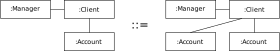
\includegraphics[width=0.75\textwidth]{grammar_rule_example}
	\caption{Graph grammar rule example: Add account}
	\label{fig:graph-grammar-rule-add-account}
\end{figure}

\noindent
A graph grammar rule describes a certain given structure within a graph which is allowed to be replaced by another structure. Fig. \ref{fig:graph-grammar-rule-add-account} illustrates an example for such a graph grammer rule. These rules are called \textit{graph rewriting rules} as well. Every rectangle within Fig. \ref{fig:graph-grammar-rule-add-account} represents a vertex and the connections between the rectangles are the edges of the graph. The left side of the rule is called the \textit{left-hand side} (LHS) graph whereas the right side of the rule is called \textit{right-hand side} (RHS) graph. This graph rewriting rule describes a simplified transformation according to the Henshin example in the last section. Whenever a manager vertex is adjacent with a client vertex which itself is adjacent with an account vertex in a graph or part of a graph, the LHS graph of the rule matches and the rule can be applied. Applying the rule adds another account vertex to the graph to which the rule is applied and connects the added vertex with the client vertex. 

\subsection{Transformation Fundamentals}
The graph grammar example above may already provide some kind of intuition of how a model transformation based on graphs can be implemented by applying multiple graph grammar rules onto an existing graph. This section aims to present the concepts behind such graph grammar based transformations in a formal manner. Note that all the following definitions and formalizations are based on the work of Ehrig et al. \cite{DBLP:series/eatcs/EhrigEPT06} and are not accomplished by this paper.

A simple graph with vertices and edges is not sufficient to model a transformation using such a rule as shown in Fig. \ref{fig:graph-grammar-rule-add-account}. The vertices and edges have to be typed in order to create such a rule. Concretely, a \textit{manager} vertex for example, differs from a \textit{client} vertex by its type. 

\begin{definition}[Graph]
A graph $G(V,E,s,t)$ consists of a set V of vertices, a set E of edges, source and target functions $s,t : E \to V$.
\end{definition}

\noindent
In order to formalize such a transformation, a so-called \textit{typed graph} is needed. A typed graph supplements a graph with types for all edges and vertices. This is actually realized with another additional graph. In addition to a given graph $G$ a so-called \textit{type graph} $TG$ is needed, which provides the types of all vertices and edges of $G$.

\begin{definition}[Type Graph]
A type graph is a graph $TG = (V_{TG},E_{TG},s_{TG},t_{TG})$.
\end{definition}

\noindent
Hence, the two graphs have to be connected in order to assign every vertex and edge in graph $G$ the according vertices and edges in the type graph $TG$. Mathematically this is solved with a graph morphism. A graph morphism defines two functions. One function maps the vertices of a graph to the other graph and the second function does the same thing with the edges.

\begin{definition}[Graph Morphism]
A graph morphism is an application $f : G_1 \to G_2$, $f = (f_V,f_E)$ of a graph $G_1$ to another graph $G_2$ which consists of two functions $f_V : V_1 \to V_2$ and $f_E : E_1 \to E_2$.
\end{definition}

\noindent
Having a graph $G$, a type graph $TG$ and such a graph morphism from $G$ to $TG$ it is possible to define the needed typed graph $G^T$.

\begin{definition}[Typed Graph]\label{typed-graph}
A typed graph $G^T = (G,f_{type})$ over a type graph $TG$ is a graph $G$ and a graph morphism $f_{type} : G \to TG$.
\end{definition}

\noindent
Fig. \ref{fig:example-graph-morphism} illustrates these definition of a typed graph applied to the example with the already introduced banking meta-model. The upper graph shows the type graph $TG$ while the lower graph represents an example for a graph $G$. The dashed arrows illustrate the graph morphism $f_{type} : G \to TG$. Note that the graph grammar rule previously shown in Fig. \ref{fig:graph-grammar-rule-add-account} actually consists of two such typed graphs even if it is not explicitely show.

\begin{figure}[H]
	\centering
	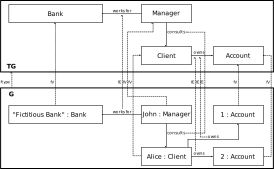
\includegraphics[width=0.95\textwidth]{example_graph_morphism}
	\caption{Example: Typed graph $G^T = (G,f_{type})$ over type graph $TG$}
	\label{fig:example-graph-morphism}
\end{figure}

\noindent
Graph rewriting rules as seen in Fig. \ref{fig:graph-grammar-rule-add-account} are also called graph productions, especially in the mathematical context. Such rules are defined by a pair of graphs LHS and RHS, as already mentioned. The LHS graph represents the preconditions which have to match a certain graph which should be transformed. The RHS represents the postconditions of the rule or 'how the graph should look like' after the transformation. However, for a graph production, a third graph $K$ called the gluing graph has to be deduced. This graph is derived by the mapping between the LHS and RHS graph. This mapping is not explicitely visible within the grammar rule, but as already explained in the Henshin example, the mapping between the LHS and RHS graph has to be provided. It defines the \textit{preserved} vertices and edges and is also implicitely 	existing in the grammar rule in Fig. \ref{fig:graph-grammar-rule-add-account} (for example it is clear that the \textit{manager} vertex in the LHS graph must be the same vertex as the \textit{manager} vertex in the RHS graph).

\begin{definition}[Graph Production]\label{graph-production}
A graph production $p = (LHS \xleftarrow{\text{l}} K \xrightarrow{\text{r}} RHS)$ consists of (typed) graphs LHS, K and RHS, and injective (typed) graph morphisms $l$ and $r$.
\end{definition}

\noindent
In order to transform a graph $G$ into another graph $G'$ given a production $p$ a procedure to actually perform the transformation, or mathematically an operator, is needed. The crucial concept used for this problem in algebraic graph transformation \cite{DBLP:series/eatcs/EhrigEPT06} is the so-called \textit{pushout}. The pushout concept is part of the category theory \cite{MAHFOUDH2015212,barr1990category}. However, explaining this theory in detail would be beyond the scope of this paper, but the definition of a pushout and a graphical intuition (Fig. \ref{fig:example-graph-pushout}) how this is applied to graphs is given.

\begin{definition}[Pushout]\label{def-pushout}
	A pushout $PO$ over two graph morphisms $f : G_1 \to G_2$ and $g : G_1 \to G_3$ is defined by a pushout graph $G_4$ and morphisms $f' : G_3 \to G_4$ and $g' : G_2 \to G_4$ with $f' \circ g = g' \circ f$.
\end{definition}

\begin{figure}[H]
	\centering
	
\includegraphics[width=0.5\textwidth]{pushout_graph}
	\caption{Graphical intuition of a pushout (Definition \ref{def-pushout}) \cite{tutorial-agt}}
	\label{fig:example-graph-pushout}
\end{figure}

\noindent
Note that three different pushout approaches exist and this papers refers to the so-called \textit{Single Pushout} (SPO)\cite{LOWE1993181}. Transformation systems may also use the \textit{Double Pushout} (DPO) approach \cite{10.1007/BFb0025714} or the \textit{High Level Replacement} (HLR) approach \cite{EHPP04} which are not introduced here. 

\noindent
The single pushout (SPO) method applied to a graph $G$ can be summarized as follows \cite{MAHFOUDH2015212}:
\begin{enumerate}
	\item Find a match of $LHS$ in $G$, or formally, find a morphism $m : LHS \to G$.
	\item Deleting the sub-graph $m(LHS) - m(LHS \cap RHS)$ from $G$, which trivially removes all elements from the graph that are within the LHS graph but not in the intersection graph of the LHS and RHS graph and thus are meant to be deleted by the rewriting rule.
	\item Adding the sub-graph $m(RHS) - m(LHS \cap RHS)$ to $G$ to get the result $G'$. This step adds all elements which are part of the RHS graph but not part of the intersection of the LHS and RHS graph and thus are meant to be created in $G'$ by the rewriting rule.
\end{enumerate}

\noindent
Note that Definition \ref{def-pushout} and Fig. \ref{fig:example-graph-pushout} describe the universal concept of a pushout. Mapped to the single pushout procedure in the graph transformation context, as described above, the graph $G_1$ would be the $LHS$ graph, $G_2$ the $RHS$ graph, $G_3$ the input graph $G$ and $G_4$ the resulting output graph $G'$.

The given graph productions (Definition \ref{graph-production}) together with a pushout operator $PO$ (Definition \ref{def-pushout}) are used to realize graph transformations. A \textit{direct (typed) graph transformation} applies a single production $p$ to a graph $G$ using the pushout $PO$, if a morphism $m : LHS \to G$ can be found (matching of the LHS). 

\begin{definition}[Direct (Typed) Graph Transformation]\label{tgt}
A direct (typed) graph transformation $G \xRightarrow{\text{p,m}} G'$ is given by $POs$, a production $p$ and match $m : LHS \to G$.
\end{definition}

\noindent
While a \textit{direct (typed) graph transformation} applies exactly one production, the term \textit{(typed) graph transformations} is used if a whole sequence of productions is applied.

\begin{definition}[(Typed) Graph Transformation]
A (typed) graph transformation $G_0 \xRightarrow{*} G_n$ is a sequence $G_0 \Rightarrow G_1$ ... $\Rightarrow G_n$ of direct (typed) graph transformations.
\end{definition}

\noindent
Fig. \ref{fig:banking-example-pushout} illustrates the theory explained above on the banking example. The graph rewriting rule  should again be used to add an additional bank account to a bank customer. 

\begin{figure}[H]
	\centering
	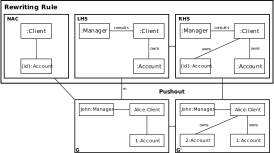
\includegraphics[width=0.9\textwidth]{banking-example-pushout}
	\caption{Banking example: rewriting rule with single pushout}
	\label{fig:banking-example-pushout}
\end{figure}

\noindent
Besides the four graphs $LHS$, $RHS$, $G$ and $G'$ illustrating the pushout principle, the rewriting rule in Fig. \ref{fig:banking-example-pushout} contains a \textit{negative application condition} (NAC) graph. This concept is also considered within the algebraic graph transformation concepts, but not formally introduced at this point. Whereas the LHS part reflects the matching function $m : LHS \to G$, this NAC represents a graph which must not match the corresponding graph $G$. If the NAC matches, the rule is in fact not applicable. Within this example the NAC graph ensures that no account with an already existing identifier is created. However, the upper part of Fig. \ref{fig:banking-example-pushout} shows the rewriting rule already introduced. The graph $G$ represents a concrete example with the manager John which consults the customer Alice. Alice already has a bank account and by the application of the rewriting rule she is getting a second account.

Given the presented definitions it is possible to formally define the term of a \textit{graph transformation system} (GTS). It is built by a type graph $TG$ and a set of graph productions $p$ which can be described as graph rewriting rules.

\begin{definition}[(Typed) Graph Transformation System]\label{gts}
A (typed) graph transformation system $GTS = (TG,P)$ consists of a type graph $TG$ and a set of (typed) graph productions $P$.
\end{definition}

\noindent
Further, it is now possible to formally define a graph grammar $GG$. A graph grammar is built with a graph grammar system $GTS$ (Definition \ref{gts}) and a start graph $S$. 

\begin{definition}[(Typed) Graph Grammar]
A (typed) graph grammar $GG = (GTS,S)$ consists of a graph transformation system $GTS$ and a (typed) start graph $S$\footnote{The start graph $S$ is a typed graph, see Definition \ref{typed-graph}.}.
\end{definition}

\begin{figure}[H]
	\centering
	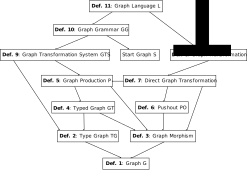
\includegraphics[width=0.80\textwidth]{definitions-graph}
	\caption{Graph Grammar \& Graph Language (Definition Dependencies)}
	\label{fig:definitions-graph}
\end{figure}

\noindent
On the basis of a graph grammar $GG$ it is possible to define a graph language $L$. Note that the start graph for a graph grammar is the same concept as the start variable you may know from string grammars.

\begin{definition}[(Typed) Graph Language]
A (typed) graph language $L$ based on a graph grammar $GG$ is defined by $L = $ \{ $G \mid \exists$ (typed) graph transformation $S \xRightarrow{*} G$ \}.
\end{definition}

\noindent
The dependencies of all presented definitions and how they build a graph grammar is illustrated in Fig. \ref{fig:definitions-graph}.

The presented algebraic graph transformation approach further allows one to reason formally about applicability of a production $p$ on a graph $G$. Ehrig et al. \cite{DBLP:series/eatcs/EhrigEPT06} also describe how to analyze if productions are parallel independet or not. This is crutial when it comes to the topic of performance and big models have to be processed. Having a good model with parallel independet productions allows parallelism and concurrency within the execution of graph transformation. Further it is possible to find so-called \textit{critical pairs}, pairs of direct transformations which are parallel dependent and thus may lead to problems during the execution of a transformation system.

Another challenge is the handling of non-determinism as soon as a set of transformation rules is applied \cite{taentzer2005model}. Non-determinism occurs if more than one rule is applicable and one of them is arbitrarily chosen. Another possible reason for non-determinism arises if a certain applied rule leads to multiple matches in the graph. There are techniques providing the possibility to indroduce a control flow to somehow reduce these kind of arbitrary choices. The problem can further be addressed by using input parameters and additional conditions in the rules in order to reduce non-determinism. Henshin addresses this problem with its control flow units introduced in Section \ref{henshin-meta-model}.

\subsection{Other Approaches}
An extended concept of the presented typed graph transformations are typed \textit{attributed} graph transformations \cite{10.1007/978-3-540-30203-2_13}. One approach which is actually using typed attributed graphs is the attributed graph grammar system AGG \cite{agg}, allowing a graph to be attributed by Java objects. AGG is a development environment for graph transformation which in comparison to Henshin requires much more knowledge of the algebraic theories from the user. However, since AGG is based on algebraic graph transformation as well, it is possible to transform a Henshin transformation model into AGG.

Another closely related concept are triple graph grammars (TGG) \cite{Schurr:1994:SGT:647675.731658}. The main advantage of this concept is the possibility to execute a transformation in both directions, despite the declarative transformation specification. Further, they allow the definition of a relation between two different models. A transformation using TGGs maintains the consistency of those two models, meaning if one model is transformed, the other model is transformed accordingly. This is possible since a TGG rule consists of three separate graphs, a source, a target and a correspondence graph.

Fig. \ref{fig:tgg-example} shows the notorious example for TGGs. Two models, one modeling packages and classes and the other modeling the corresponding database schema with its tables. The correspondence model in between synchronizes the two models and keeps them consistent. Atom\textsuperscript{3} \cite{taentzer2005model,10.1007/3-540-45923-5_12} is one approach providing a tool for model transformation with TGGs.

\begin{figure}[H]
	\centering
	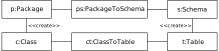
\includegraphics[width=0.6\textwidth]{tgg-example}
	\caption{TGG example: Two synchronised models with correspondence graph \cite{DBLP:phd/de/Konigs2009}}
	\label{fig:tgg-example}
\end{figure}

\noindent
Besides the already mentioned approaches which are fully based on algebraic graph transformations, other approaches relying on different theories exist. An example is the VIATRA \cite{viatra} approach which combines graph transformation with the formal paradigm of abstract state machines (ASM) \cite{Borger:2003:ASM:829603}.

After the introduction into the graph transformation fundamentals and theories within this section, we return to the practical applications. The next section is going to show how model transformation can be applied to DSL processing.

\section{Towards DSL Processing}\label{dsl-processing}
Models can be represended in various ways. Often they are represented in graphical notations such as the Unified Modeling Language (UML) or simply in code. However, sometimes these approaches do not suit ideally, for example if the usability is not sufficient. In such a case it might be a better solution to come up with a new representation which is specifically developed for the actual problem domain.

\subsection{Domain-specific Languages (DSL)}
Domain-specific Languages (DSL) are languages which are implemented for a specific domain, as the name DSL already implies. In contrast to General Purpose Languages (GPLs) such as C, C++ or Java, DSLs are very limited in their features. GPLs are not limited to a certain problem domain and are used for implementing systems of any kind, whereas DSLs aim to improve the software development process within a specific and restricted scope. On one hand this can improve the productivity for developers, since it is easier to describe the structure and behavior of the domain in the specific language and on the other hand it might improve the communication between developers and domain experts because the language is much easier to read \cite{Fowler:2010:DSL:1809745}.

DSLs are used to define models in a certain representation. The parser of a DSL reads the text written in the defined syntax and generates a semantic model, the model which is populated by the DSL \cite{Fowler:2010:DSL:1809745}. The model can then be processed further. Often DSLs are used to generate code in a GPL, which is basically a model-to-code transformation with the semantic model of the DSL as input. Nevertheless, DSLs are not limited to this kind of application. They can be used for designing and modeling sofware architectures as well, also mentioned as Architecture DSLs (ADSLs) in \cite{Voelter}, or for requirements engineering purposes. As already explained in the beginning of this paper, models can be used in all software engineering disciplines.

\subsection{DSL Processing with Model Transformation}
As previously mentioned, a DSL and the concrete instances written in a DSL are generally developed to somehow process them further. Besides generating code or applying any other exogenous transformation, it might be interesting to apply refactorings to your DSL. Further, architectural refactorings \cite{ZimmermannArchitecturalRefactorings} could be applied if the DSL describes the architecture of a software.

This brings us back to model transformation since any processing of a DSL can be implemented with this concept. A concrete DSL instance can be parsed and therefore processed into an model instance of the semantic model (meta-model) behind the language. Obviously it is then possible to apply a model transformation to that model. As long as the transformed target model is still based on the same meta-model (the semantic model of the DSL) it can be converted back to the syntax of the DSL.

The next section explains a concrete example of this process using Henshin and a DSL based on Xtext. Xtext is one of the most widespread technologies for implementing external DSLs. It further suits well for implementing DSL processing as explained above, since the meta-model of the semantic model produced by Xtext is the Ecore model, which is used by many model transformation tools such as Henshin. The process for the following example can be summarized as follows:
\begin{enumerate}
	\item A Xtext-based DSL instance is parsed by the Xtext parser which creates an Ecore model.
	\item Henshin is used to apply a model transformation to that Ecore model.
	\item The transformed Ecore model is then converted back to the DSL syntax.
\end{enumerate}

\subsection{Example: A DSL for Service Decomposition}\label{example-dsl}
This example is based on the ContextMapper\footnote{\url{https://contextmapper.github.io/}} DSL \cite{context-mapper}, a DSL for service decomposition \cite{dsl-for-service-decomposition}. The language allows to model context maps based on strategic Domain-driven Design (DDD) patterns. In a future project the DSL should be used to realize a tool calculating service decomposition proposals as a series of architectural refactorings \cite{ZimmermannArchitecturalRefactorings} based on model transformations. Note that this example is simplified and only a little part of the DSL semantic model is used. The whole model actually covers almost all DDD patterns, strategic and tactic. This example is reduced to the patterns \textit{Bounded Context}, \textit{Aggregate} and \textit{Entity}. 

\lstset{
	caption={Example Input: Bounded Contexts specified with ContextMapper DSL},
	label=context-mapper-dsl-input,
	basicstyle=\tiny,
	morekeywords={BoundedContext, Aggregate, Entity},
	frame=single
}
\begin{lstlisting}
BoundedContext CustomerManagement {
  Aggregate Customers {
    Entity Customer{
      String firstName
      String familyName
      Account customerBankAccount
    }
    Entity Account {
      String iban
      String bankName
    }
  } 
  Aggregate CustomerSelfService {
    Entity Account {
      String username
      String password
      Customer owner
    }
  }
}
\end{lstlisting}

\noindent
A bounded context implements one or multiple aggregates and each aggregate can then contain multiple entities. For details regarding these patterns please consult the according literature \cite{EvansEric2012Dd:t,Vernon:2013:IDD:2462636,millett2015patterns,dsl-for-service-decomposition}. Listing \ref{context-mapper-dsl-input} shows an example of a bounded context modeled with the ContextMapper DSL.

Service decomposition deals with the problem how services, or in terms of DDD, how bounded contexts should be splitted. One possible indicator that a bounded context should be splitted is the existence of a \textit{same term with different meanings} \cite{brandolini-infoq}. The following transformation implements a simplified architectural refactoring \cite{ZimmermannArchitecturalRefactorings} for such a case. Listing \ref{context-mapper-dsl-input} shows a bounded context which implements two aggregates. These aggregates both include an entity called \textit{Account}. Once it means the bank account of a customer and in the other case the user account for the self-service application login (the same term for different meanings). The refactoring should split such a bounded context into two. This means the resulting context map should contain two bounded contexts, each of them containing one of the existing aggregates.

\begin{figure}[H]
	\centering
	\includegraphics[width=1.0\textwidth]{ContextMapRefactoring_Example}
	\caption{Example: Split Bounded Context Transformation Rule}
	\label{fig:context-map-refactoring-henshin}
\end{figure}

\noindent
Figure \ref{fig:context-map-refactoring-henshin} illustrates the refactoring, implemented with Henshin. To simplify the example, the name of the entity by which the refactoring should split the context is given as a parameter. The LHS graph matches a bounded context with two aggregates, each one containing an entity with the name given by the parameter. The RHS graph does not contain one of the two edges connecting the bounded context with its aggregates, which disconnects one aggregate from the existing bounded context. Note that it is somehow non-deterministic which aggregate moves to the new bounded context within this example. Further, the RHS graph contains a new bounded context named \textit{SplitBoundedContext} which is connected to the \textit{moving} aggregate with a new edge.

Another additional edge adds the bounded context to the context map. Applying this Henshin transformation to the example model from Listing \ref{context-mapper-dsl-input} leads to the following result shown in Listing \ref{context-mapper-dsl-output}.

\lstset{
	caption={Example Output: Bounded Contexts specified with ContextMapper DSL},
	label=context-mapper-dsl-output,
	basicstyle=\tiny,
	morekeywords={BoundedContext, Aggregate, Entity},
	frame=single
}
\begin{lstlisting}
BoundedContext CustomerManagement {
  Aggregate Customers {
    Entity Customer{
      String firstName
      String familyName
      Account customerBankAccount
    }
    Entity Account {
      String iban
      String bankName
    }
  } 
}
BoundedContext SplitBoundedContext {
  Aggregate CustomerSelfService {
    Entity Account {
      String username
      String password
      Customer owner
    }
  }
}
\end{lstlisting}

\noindent
The two entities with the same name are now distributed to two separate bounded contexts. Of course the example is kept very simple and needs to be enhanced for a productive refactoring tool. However, it is a good illustration how model transformation can be used for processing DSLs.

\section{Related Work}\label{tools}
This section is giving an overview over other tools and approaches and compares them with the Henshin approach.

\subsection{Graph-based Approaches}
A closely related approach is AGG \cite{agg}, as already mentioned. Similar to Henshin it is based on an algebraic approach. Further, it works with attributed typed graphs and allows to attribute a graph with Java objects. However, AGG \cite{agg} is a quite theoretic research project and the usage of the engine demands a higher effort to implement a transformation in practice. It can be seen as a low-level framework or engine for algebraic graph transformation. Actually, EMF Tiger \cite{emf-tiger} which is the predecessor of Henshin is based on AGG. Thus, all of these three approaches are based on the same theory, but Henshin which has enhanced the EMF Tiger approach is the most modern and most mature tool of the three. Since it is based on EMF Ecore models it benefits from the broad spectrum of available tools arround the EMF framework which makes it easy to model the transformation input. Further, a Henshin transformation can be converted to AGG if it is needed for deeper analysis and verifications.

\subsection{Other Tools}
Model transformation tools typically differ from the others by in the technical space and the type of transformation (in-place or out-place) they realize. In the case of Henshin \cite{Arendt:2010:HAC:1926458.1926471} and EMF Tiger \cite{emf-tiger} this would be the EMF framework. Other EMF-based approaches are Kermeta \cite{kermeta}, Mola \cite{mola}, Fujaba \cite{fujaba}, Moment2 \cite{moment2} and the Epsilon Transformation Language (ETL) \cite{etl}, which all have in common that they implement in-place transformations. 

Representative out-place approaches are QVT \cite{qvt}, ATL \cite{atl} and Tefkat \cite{tefkat}. QVT \cite{qvt} is a specification of the Object Management Group (OMG) and part of their Meta Object Facility (MOF) \cite{mof}. ATL \cite{atl} is an Eclipse-based toolkit and provides a huge scenario catalog for exogenous out-place transformations with their transformations zoo. Tefkat \cite{tefkat} uses the EMF framework in their out-place transformation implementation. Since the goal of this paper is to show an example of in-place transformation for DSL processing and the DSL is based on Xtext, the tool selection was reduced to EMF Ecore-based in-place transformation tools. Thus, this section will not discuss the other tools and approaches further.

Kermeta provides an imperative action language for implementing model transformations, which is a completely different approach in comparison to Henshin. The transformation has to be implemented in an imperative style and is not based on rules. Thus, no formal foundation exists. A similar approach is provided by ETL. Even though it is rule-based, the implementation of a rule is given in an imperative style. Mola transformations can be specified with a graphical tool resulting in so-called Mola diagrams. It is based on pattern-matching and rules. However, those are specified by traditional programming concepts such as loops, branching and calls to subprograms. There is no basis for a formal validation of a transformation. Fujaba is an acronym for \textit{'From UML to Java and back again'} which already indicates that the Fujaba tool was invented for rather specific transformations. But it provided a feature to specify model-to-model transformations based on triple graph grammars (TGG). However, the project seem to be out-dated and no longer maintained. Moment2 provides transformations based on a rewriting logic concept similar to graph transformation. Further, it is possible to formally verify and analyze its transformations. The major drawback is that these rewrites cannot be composed to a larger transformation system.

\subsection{Summary}
In summary, Henshin seems to be the only EMF-based tool which does not only provide the formal foundations based on algebraic graph transformations, but also provide tools and a Java API which are mature enough to use in the practical field as well. In comparison to many others, the transformation system and its rules are specified with an Ecore-based model in a rather declarative instead of an imperative way. The formal foundations might not only be interesting for research but in practice as well as soon as it comes to analysis and verification of a transformation system.

\section{Conclusion}
In this paper we introduced the term \textit{model transformation} and its characteristics. We further compared it with the term \textit{program transformation} and concluded that program transformations can be seen or implemented as \textit{code-to-code} model transformations. In addition, we illustrated how a model transformation approach can be applied to DSL processing. A proof of concept using the Context Mapper DSL \cite{context-mapper} has been implemented to demonstrate how the approach can be used to implement architectural refactorings \cite{ZimmermannArchitecturalRefactorings} on the basis of a DSL.

To implement this approach as shown in Section \ref{dsl-processing}, the Henshin transformation tool has been used. We further introduced its concepts and the theories behind it. By implementing the presented examples, we evaluated the tool and compared it with other available approaches. 

To summarize, the Henshin tool seems to be one of the most mature model transformation tools, especially in the Ecore universe. Besides the usability issues regarding the Eclipse UIs, we have not faced any problems and were able to implement the DSL example transformation within a few hours. The tool is documented well and we got used to it quickly. The declarative approach of specifying the transformation rules with the automatically generated graphical diagram provides a good expressiveness in comparison with other rather imperative approaches. Note that the presented formal theories behind the approach are not needed as a user of the tool. However, due to the solid foundations behind Henshin it is possible to formally reason about the implemented transformations which might be helpful if the implemented transformation systems are getting complex. 

\newpage
\bibliographystyle{splncs04}
\bibliography{paper}

\end{document}
